\documentclass[letterpaper]{article}
\usepackage{listings}
\usepackage{booktabs}
\usepackage{array}
\usepackage{multirow}
\usepackage{amsmath,amssymb}
\usepackage{hhline}
\usepackage{authblk}
\usepackage[T1]{fontenc}
\usepackage{lipsum}
\usepackage{float}  
\usepackage{graphicx}
\usepackage[export]{adjustbox}
\usepackage{caption}
\usepackage{subcaption}
\usepackage[final]{pdfpages}
\usepackage{wrapfig}
\renewcommand{\baselinestretch}{2}

\usepackage[letterpaper, margin=1in]{geometry}

\begin{document}

\title{Train Controller User Manual}
\author{Michael Ghaben}
\date{}

\maketitle


\section{Track Model}

\subsection{UI Layout}
\begin{figure}[h]
	\centering
	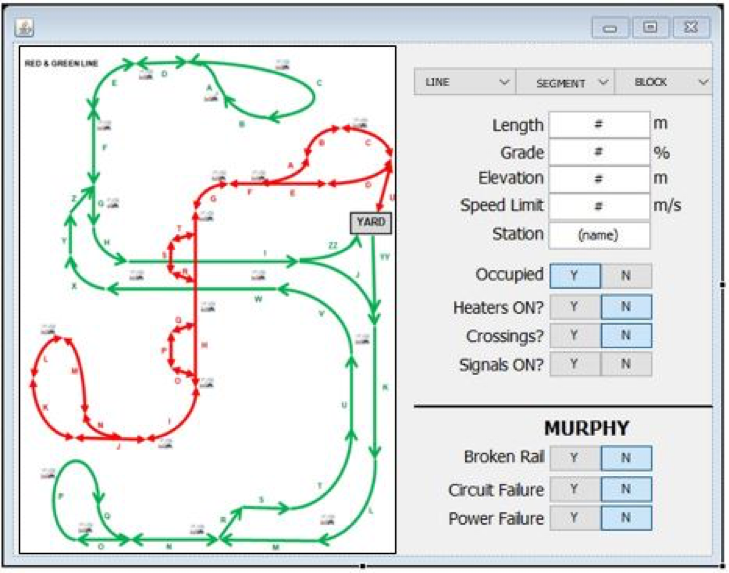
\includegraphics{trackUI.PNG}
	\caption{The current Track UI layoutl}
\end{figure}


\subsection{UI Buttons and Actions}

	\subsubsection{Line, Section, and Block Selection}
		\begin{itemize}
			\item Line Selection - The user may select the line to view from the "line" dropdown list of lines 
			\item Section - The user may select the section to view from the "section" dropdown menu
			\item Block - The user may select the block from the block dropdown menu
		\end{itemize}
		After selecting the Line / Section / Block, the user may view the pertinent information on the panels of the screen.
	\subsubsection{Static Information}
	The user may view the static information about the track on the righthand panel. This information will be loaded into the program via an excel file at initialization. The following information is displayed:
		\begin{itemize}
			\item Length - The length of the selected block (feet)
			\item Incline / Grade - The grade of the selected block (percent)
			\item Elevation - The elevation of the selected block (feet)
			\item Speed Limit - The speed limit of the selected block (miles per hour)
			\item Station - If a station is on this block, a station name will be given. If there is no station on the block, this field will be empty
		\end{itemize}
		The values will be provided in imperial units. Furthermore, the track direction and infrastructure (such as underground) will be reflected in the graphical display on the left. Track direction will be marked with the arrows as shown, and infrastructure will be marked via a drawing scheme. Switches will be marked graphically with an "open" or "cllosed" on the map between the sections which are connected.
	
\subsection{Dynamic Information}
		Additionally, the following dynamic information will be provided based upon the runtime environment of the train system:
		\begin{itemize}
			\item Occupied - Is the selected block of the track occupied
			\item Heaters - If the selected block has heaters, are they on?
			\item Crossings - Are railway crossings down? ("Yes" implies the railway crosisngs are down)
			\item Signals ON - Are the train light signals currently on?
		\end{itemize}
		The railway crossings terminology may be chagned as to make the information presented clearer.

\subsection{User Control}
In this module, no control of the tracks state from the external user interface is provided. This is a reflection of the underlying philosophy that the track model itself should be "dropped out" and replaced by a physical track when the end user (the train company). In this case, the track models primary duties -- loading passengers onto the track and turning the heaters on and off -- will be handled automatically, with the ability to programmatically control the variables. 

\end{document}